\documentclass{article}
\usepackage{listings}
\usepackage{graphicx}
\usepackage{color}
\usepackage{pgfplots}
\usepackage{float}
\usepackage{multirow}
\pgfplotsset{compat=1.18}
\usepackage[margin=0.75in]{geometry}
\definecolor{dkgreen}{rgb}{0,0.6,0}
\definecolor{gray}{rgb}{0.5,0.5,0.5}
\definecolor{mauve}{rgb}{0.58,0,0.82}
\lstset{,
  language=C++,
  aboveskip=3mm,
  belowskip=3mm,
  showstringspaces=false,
  columns=flexible,
  basicstyle={\small\ttfamily},
  numbers=none,
  numberstyle=\tiny\color{gray},
  keywordstyle=\color{blue},
  commentstyle=\color{dkgreen},
  stringstyle=\color{mauve},
  breaklines=true,
  breakatwhitespace=true,
  tabsize=3
}
\title{Assignment 5}
\author{Bhavya[U21CS100], Garvit[U21CS089], Swayam[U21CS079]}
\begin{document}
    \maketitle
    
    \section{Tiling Problem}
    \subsection{Question}
    Consider the following tiling problem. We have a courtyard with 2$^n$ x 2$^n$ squares and 
    we need to tile the courtyard using L-shaped tiles or trominoes. Each trominoe consists 
    of three square tiles attached to form an L shape as shown below.
\\    

    Can this be done without spilling over the boundaries, breaking a tromino or having 
    overlapping trominoes? The answer is no, simply because 2$^n$ x 2$^n$ = 2$^{2n}$ is not divisible by 3, 
    only by 2. However, if there is one square that can be left untiled, then 2$^{2n}$ - 1 is 
    divisible by 3. Can you show this?
\\       

    Is there an algorithm that tiles any 2$^n$ x 2$^n$ courtyard with one missing square in an arbitrary 
    location? As an example, below is a 2$^3$ x 2$^3$ where the missing square is marked "O". Does the 
    location of the missing square matter?
\\

\begin{figure}[h]
  \centering
  \includegraphics[width=0.5\textwidth]{/Users/garvitshah/Desktop/College/Current-Sem/Subjects/DAA/Mini Project/jjkk.png}
  \caption{8x8 Courtyard}
  \label{fig:example}
\end{figure}



    \subsection{Input Format:}
        Matrix Size - $n$\\
        Position of the Statue - $x$ $y$\\
    \\


     \newpage
     \section{Solution}
     \subsection{Algorithm}
     \begin{enumerate}
     \item Define the courtyard as a rectangular grid of cells.
     \item Define the L-shaped tile as a set of 4 squares, each with a boolean value indicating whether the square is filled or not.
     \item Generate all possible orientations of the L-shaped tile (there are 8 possible orientations, including rotations and reflections).
     \item For each cell in the courtyard, attempt to place the L-shaped tile in each of its possible orientations, one at a time, checking if the tile fits and does not overlap with any other tiles already placed.
     \item If a tile fits and does not overlap, mark the cells covered by the tile as filled.
     \item Repeat step 4 and 5 for all remaining cells in the courtyard until the entire courtyard is covered or no more tiles can be placed.
     \item If the entire courtyard is covered without any overlapping tiles, then the problem is solved. Otherwise, the problem has no solution.
     \end{enumerate}
     
     \newpage
     \subsection{Psuedo Code}{Divide and Conquer Apporach}

     \begin{lstlisting}
      // grid is the given 2$^n$ x 2$^n$ grid initialised with all zero
      // pos is the position of the statue on the grid given in the form of (x,y)
      // N is the number to be placed as tile group

      tiling(grid, x, y, N, statue.x, statue.y){
        pos(x, y)
        posvector[][]
        if (N != 0){
          m = pow(2, N-1)
          if (statue.x >= m and statue.y < m){
            pos2 = tiling(grid, x, y, n-1, m - 1, m - 1)
            pos = tiling(grid, x + m, y, n-1, statue.x- m, statue.y)
            pos3 = tiling(grid, x, y + m, n-1, m - 1, 0)
            pos4 = tiling(grid, x + m, y + m, n-1, 0, 0)
            posvector.push_back(pos2)
            posvector.push_back(pos3)
            posvector.push_back(pos4)
          }  
          else if (statue.x < m and statue.y < m){
              position pos4 = tiling(grid, x + m, y + m, n-1, 0, 0)
              position pos3 = tiling(grid, x, y + m, n-1, m - 1, 0)
              position pos1 = tiling(grid, x + m, y, n-1, 0, m - 1)
              pos = tiling(grid, x, y, n-1, statue.x, statue.y)
              posvector.push_back(pos3)
              posvector.push_back(pos4)
              posvector.push_back(pos1) 
          }     
          else if(statue.x < m and statue.y >=m){
              pos2 = tiling(grid, x, y, n-1, m - 1, m - 1)
              pos1 = tiling(grid, x + m, y, n-1, 0, m - 1)
              pos = tiling(grid, x, y + m, n-1, statue.x, statue.y-m)
              position pos4 = tiling(x + m, y + m, n-1, 0, 0)
              posvector.push_back(pos2)
              posvector.push_back(pos4)
              posvector.push_back(pos1)
          }
          else if(statue.x >= m and statue.y >= m){
              pos2 = tiling(grid, x, y, n-1, m - 1, m - 1);
              pos3 = tiling(grid, x, y + m, n-1, m - 1, 0);
              pos1 = tiling(grid, x + m, y, n-1, 0, m - 1);
              pos = tiling(grid, x + m, y + m, n-1, statue.x - m, statue.y - m);
              posvector.push_back(pos2);
              posvector.push_back(pos3);
              posvector.push_back(pos1);
          }
        
          tilenum = tilenum + 1;
          for i = 0 till i = 3
          {
            matrix[(posvector[i]).y][(posvector[i]).x] = tilenum;
          }
        }
      return pos;
  
}  


       \end{lstlisting} 
    
    \newpage
    \subsection{C++ Code}
    \begin{lstlisting}
    #include<iostream>
    #include<cmath>
    #include<vector>
    #include <time.h>

    int matrix[8][8] = {{0},{0}};
    int tilenum = 0;
    class position{
        public:
        int x;
        int y;

        position(int x, int y)
        {
            this->x = x;
            this->y = y;
        }
    };

    position tiling(int x, int y, int n, int b1, int b2)
    {
        position pos(x, y);
        std::vector<position> posvector;
        if(n!=0)
        {
            int m = pow(2,n-1);
            if((b1>=(m)) && (b2<(m)))//Bill is in quadrant 1
            {   
                position pos2 = tiling(x, y, n-1, m - 1, m - 1);
                pos = tiling(x + m, y, n-1, b1- m, b2);
                position pos3 = tiling(x, y + m, n-1, m - 1, 0);
                position pos4 = tiling(x + m, y + m, n-1, 0, 0);
                posvector.push_back(pos2);
                posvector.push_back(pos3);
                posvector.push_back(pos4);

            }else if((b1<(m)) && (b2<(m)))//Bill is in quadrant 2
            {
                position pos4 = tiling(x + m, y + m, n-1, 0, 0);
                position pos3 = tiling(x, y + m, n-1, m - 1, 0);
                position pos1 = tiling(x + m, y, n-1, 0, m - 1);
                pos = tiling(x, y, n-1, b1, b2);
                posvector.push_back(pos3);
                posvector.push_back(pos4);
                posvector.push_back(pos1);
            }else if((b1<(m)) && (b2>=(m)))
            {
                position pos2 = tiling(x, y, n-1, m - 1, m - 1);
                position pos1 = tiling(x + m, y, n-1, 0, m - 1);
                pos = tiling(x, y + m, n-1, b1, b2-(m));
                position pos4 = tiling(x + m, y + m, n-1, 0, 0);
                posvector.push_back(pos2);
                posvector.push_back(pos4);
                posvector.push_back(pos1);
            }else if((b1>=(m)) && (b2>=(m)))
            {
                position pos2 = tiling(x, y, n-1, m - 1, m - 1);
                position pos3 = tiling(x, y + m, n-1, m - 1, 0);
                position pos1 = tiling(x + m, y, n-1, 0, m - 1);
                pos = tiling(x + m, y + m, n-1, b1 - m, b2 - m);
                posvector.push_back(pos2);
                posvector.push_back(pos3);
                posvector.push_back(pos1);
            }

            tilenum++;
            for(int i=0; i<3; i++)
            {
                matrix[(posvector[i]).y][(posvector[i]).x] = tilenum;
            }
        }
        return pos;
    }

    int main()
    {
      int n;
      int x,y;
      std::cout<<"Enter the value of n:"<<std::endl;
      std::cin >>n;
      std::cout<<"Enter the coordinates of statue:"<<std::endl;
      std::cin>>x>>y;
      int r = pow(2,n);
      position posBill = tiling(0, 0, n, x, y);
      matrix[(posBill).y][(posBill).x] = 100;
      for(int i=0; i<r; i++)
      {
          for(int j=0; j<r; j++)
          {
              std::cout<<matrix[i][j]<<'\t';
          }
          std::cout<<"\n\n\n";
      }
    }
    \end{lstlisting}
    
    \newpage   
    \section{Time Complexity Analysis} 
    \subsection{Recurrence Relation and Tree}
    \subsubsection{Recurrence Relation}
    Since in each recursive call, we are dividing the matrix into 4 Quadrants and the cost for combining the subproblems is constant
    the recurrence relation will be given by the following equation - 
    \\
    \begin{center}
    $T(n)$ $=$ $4*T(n/4)$ $+$ $\theta(1)$
    \end{center}

    \textbf{Assumption}: $n$ is the no. of elements in the matrix. 
    
    \subsubsection{Recurrence Tree}
    Using the above recurrence relation we can depict the following recurrence tree -
    \\
    \includegraphics[width=1\textwidth]{/Users/garvitshah/Desktop/College/Current-Sem/Subjects/DAA/Mini Project/recursion_Tree.jpg}
    \begin{table}[h!] 
      \centering     
      \begin{tabular}{ | p{3cm} | p{3cm} | }  
        \hline
       Levels & Cost\\
       \hline
       0 & $c$\\
       1 & $4^{1}*c$\\
       2 & $4^2*c$\\
       . & .\\
       . & . \\
       . & . \\
       h & $4^h*c$\\
       \hline
      \end{tabular}
   \end{table}
  
   \begin{itemize}
    \item Height of Tree \textbf{$h$ $=$ $log_{4}(n)$}
    \item Number of Nodes at level-$h$ = $4^{log_{4}(n)}$ = $n$
    \item Time Complexity = $T(n)$ = $\Theta(n)$
   \end{itemize}

   \newpage
   \subsection{Subsitution Method}
   \subsubsection{Inductive Hypothesis:} 
   From the Recursion tree shown above, we can guess the solution this problem to be :
   $\Theta(n)$
   i.e $T(n)$ $=$ $cn$.
\\

Proving the above hypothesis using Strong Induction:
 \subsubsection{Base Case:}
 For $n$ $=$ $1$,\\
 
 $T(n)$ $=$ $cn$ $=$ $c$\\
 
 also, $T(n)$ $=$ $4*T(n/4)$ $+$ $c$\\
            
 $T(n)$ $=$ $4*T(1/4)$ $+$ $c$ $=$ $c$\\
            
 Hence the hypothesis holds for the base case.
 
 \subsubsection{Recursive Case:}
 Let us assume the guess holds for all $m$ $(1,n)$ union $Z$.\\

 In that case, $T(n)$ $=$ $4*T(n/4)$ $+$ $c$,\\
 
 here we know, $1 < n/4 < n$, thus the above assumption holds for $n/4$\\

So, $T(n)$ = $4*c*(n/4)$ + $c$\\

$T(n)$ $=$ $cn$ $+$ $c$\\

Consider the modified Hypotheis as $T(n)$ $=$ $cn$ $-$ $d$\\

 thus, $C - 4d < 0$\\

 Therefore, T(n) = cn = $\Theta(n)$

 \subsection{Master Theorem}
 $T(n)$ $=$ $4*T(n/4)$ $+$ $c$\\

  $T(n)$ $=$ $4*T(n/4)$ $\Theta(1)$ $=$ $a*T(n/4)$ $+$ $f(n)$\\

  Here, $log_{b}(a)$ = $log_{4}(4)$ = 1\\
  $$n^{log_{b}(a)}=n$$

  Since f(n) = $O(n^{1-\epsilon})$ for some constant $\epsilon > 0$\\

   Therefore, $T(n)$ = $O(n)$ by the virtue of the Master Theorem

   \newpage
   \section{Graphs}
   \begin{center}
    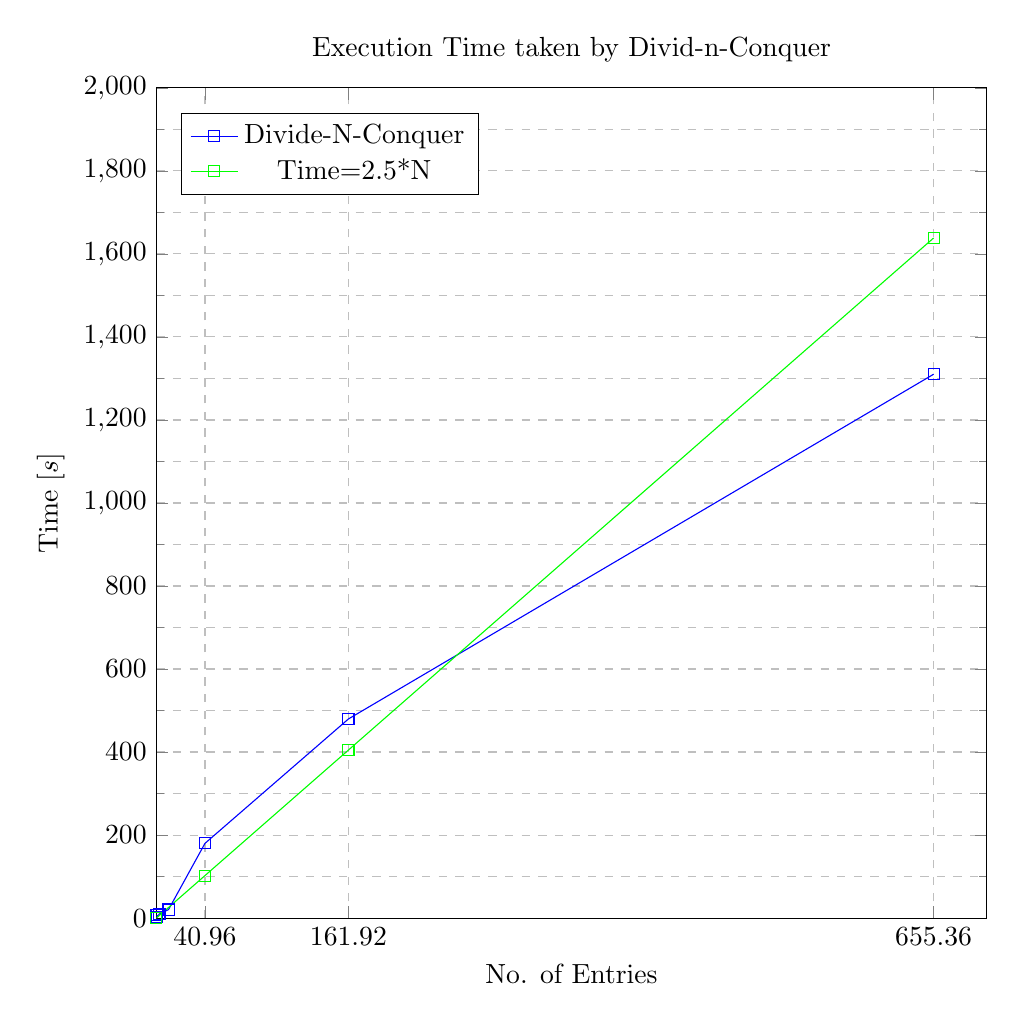
\begin{tikzpicture}
       \begin{axis}[
           title={Execution Time taken by Divid-n-Conquer},
           xlabel={No. of Entries},
           ylabel={Time [\(s\)]},
           xmin=0, xmax=700,
           ymin=0, ymax=2000,
           minor tick num = 1,
           height = \textwidth,
           width = \textwidth,
           xtick={40.96,161.92,655.36},
           ytick={},
           legend pos=north west,
           grid=both,
           grid style=dashed,
       ]
    
       \addplot[
           color=blue,
           mark=square,
           ]
           coordinates {
           (0.16,8.08)(0.64, 3.398)(2.56, 9.819)(10.24, 20.511)(40.96,180.0)(161.92,479.7)(655.36,1310.2)
           };   
        \addplot[
        color=green,
        mark=square,
        ]
        coordinates {
        (0,0)(40.96,102.4)(161.92,404.8)(655.36,1638.4)
        };        

        \legend{Divide-N-Conquer, Time=2.5*N}
       \end{axis}
       \end{tikzpicture}
    \end{center}
    

\end{document}